\documentclass[11pt,a4paper]{article}
\usepackage[T1]{fontenc}
\usepackage[margin=2.5cm]{geometry}
\usepackage{xcolor}
\usepackage{amsmath}
\usepackage{booktabs}
\usepackage{array}
\usepackage{adjustbox}
\usepackage{placeins}
\usepackage{graphicx}
\usepackage{eso-pic}
\usepackage{pgfplots}
\usepgfplotslibrary{groupplots}
\pgfplotsset{compat=1.17}
\usetikzlibrary{arrows.meta,positioning,calc}
\usepackage[numbers,sort&compress]{natbib}
\usepackage{lineno}
\usepackage[hidelinks]{hyperref}
\hypersetup{pdfauthor={}, pdftitle={A camera-referenced robotic bench method for comparing pen digitisers}}
% Build switches. The build script sets them in the file buildconfig.tex.
\newif\ifsubmission \submissionfalse
\newif\ifresultsloaded \resultsloadedfalse
\newif\ifdryrun \dryrunfalse
\newif\ifposthoc \posthocfalse
\providecommand{\resultsdir}{results}
\InputIfFileExists{buildconfig}{}{}

% An unfinished passage. The draft shows it in a red box. The submission build stops at it.
\newcounter{pendingcount}
\newcommand{\pending}[1]{%
  \ifsubmission
    \GenericError{}{Submission build: an unfinished passage remains}{Remove every unfinished passage.}{#1}%
  \else
    \stepcounter{pendingcount}%
    \par\smallskip\noindent
    {\color{red}\fbox{\parbox{\dimexpr\linewidth-2\fboxsep-2\fboxrule\relax}{\small\textbf{PENDING:} #1}}}\par\smallskip
  \fi}

% The mark of a table or figure that comes from synthetic test input.
\newcommand{\dryrunmark}{\textcolor{red}{\textbf{DRY RUN. SYNTHETIC TEST INPUT. NOT A RESULT.}}}

% A generated result file. A missing file gives a visible note in the draft and stops the submission build.
\newcommand{\resultfile}[1]{%
  \InputIfFileExists{\resultsdir/#1}{}{%
    \ifsubmission
      \GenericError{}{Submission build: the result file #1 is missing}{Run the results script.}{}%
    \else
      \pending{The generated result \texttt{\detokenize{#1}} is not available. The results script writes it from the bench analysis.}%
    \fi}}
% The same for a result that is optional in the draft.
\newcommand{\optionalresultfile}[1]{\InputIfFileExists{\resultsdir/#1}{}{}}

\newcommand{\loadresultnumbers}{%
  \InputIfFileExists{\resultsdir/numbers}{}{}%
  \ifsubmission
    \ifresultsloaded\else
      \GenericError{}{Submission build: no results are loaded}{Run the results script.}{}%
    \fi
    \ifdryrun
      \GenericError{}{Submission build: the results are a dry run}{Use the measured results.}{}%
    \fi
  \fi}

% A page mark for every draft page that holds dry-run content.
\newcommand{\dryrunwatermark}{%
  \ifdryrun
    \AddToShipoutPictureFG{\AtPageUpperLeft{\raisebox{-1.2cm}{\hspace{1.5cm}\dryrunmark}}}%
  \fi}

\loadresultnumbers
\dryrunwatermark
\title{A camera-referenced robotic bench method for comparing pen digitisers,\\ applied to an Apple Pencil and a Wacom tablet}
\author{Anonymous authors}
\date{}
\begin{document}
\maketitle
\linenumbers
% Five parts: the question; what was known; what we did; why the reader should care; why it matters.
\begin{abstract}
Do an Apple Pencil on an iPad and a pen on a Wacom tablet measure the same drawing movement?
Drawing and handwriting features are studied as health measurements, and models and reference values from one device are often applied to recordings from the other.
Earlier comparisons used people, who move differently on each surface, so the difference between the measurement chains was not known.
We built a bench in which a motion system draws the same programmed loops, spirals, and oscillating lines on both devices, while a camera at 240 frames per second measures the movement that the stylus makes.
For six features, we tested equivalence against limits that were fixed before the main runs.
Where published data allowed it, the limit is the device bias that alone gives a screening model an area under the curve of 0.55 when cases and controls use different devices.
The design has six mountings per device and 720 main runs. A cross-device correction and a simulation with generated cohorts complete the study.
\pending{State the results: which features are equivalent, the largest bias with its interval, the correction check, and the primary consequence summaries. State the tested range.}
A user of drawing features can read from these results which features transfer between the two devices, which need a correction, and how large the error of a screening model can be when devices are mixed.
The method applies to any pair of pen digitisers and gives device comparisons a mechanical reference that studies with people cannot provide.
\end{abstract}

\section{Introduction}
% Budget: title, abstract, and introduction share 1.0 page.
% Order: why device measurement agreement matters; the measurement question;
% independent motion reference; correction question; synthetic consequence question;
% four planned contributions; scope of the claim.
% Define measurement chain, feature, equivalence, and synthetic cohort.
% Contributions: bench agreement, cross-device correction, synthetic consequences,
% and release of data, capture and analysis code, programs, and fixture files.
% A release is planned. Do not assert availability before the owner sets its licence.
% Leave out claims of novelty without a checked literature search, project history,
% platform architecture, clinical utility, and conclusions about people.
\pending{Write the measurement problem, questions, contributions, and scope.}

\section{Related Work}
% Budget: 0.5 page.
% Order: earlier tablet spiral comparison (R5); writing surface effects (R6);
% sources for limits (R2, R4, R6); descriptive smoothness terminology (R3).
% Define correlation versus agreement, test-retest variation, and measurement error.
% R5 used no Apple Pencil. Correlation does not establish equivalence.
% Distinguish a source population from the bench study, which has no participants.
% Leave out unsupported absence claims and unverified references.
\pending{Compare the prior spiral study \cite{R5} with this measurement design. Explain surface effects \cite{R6}.}
\pending{Explain the roles and limits of the source measurements \cite{R2,R4,R6} and smoothness terminology \cite{R3}.}

\section{Measurement problem and design}
\label{sec:design}

\subsection{The measurement chain}
A drawing feature is the last step of a chain.
The chain has a stylus, a digitiser, an operating system, a capture application, and the analysis software.
We call it the \emph{measurement chain}.
Two chains can report different feature values for the same movement.
The cause can be the sampling rate, the timestamps, the position scale, the filtering, or the noise.

We compare two chains.
Chain P is an iPad Pro with an Apple Pencil Pro.
Chain W is a Wacom Intuos Pro tablet with its pen, connected to a computer.
The same analysis software computes the features on both chains.
For brevity, we call the two chains device P and device W.

The question has one form for each feature.
Do device P and device W give equivalent values for the same movement, within a limit fixed in advance?
\emph{Equivalent} means that the difference between the devices lies inside the limit, with stated confidence, on every tested movement.
A test that finds no difference does not show equivalence.
We therefore use an equivalence test (Section~\ref{sec:stats}).

\subsection{Why a motion system and a camera}
A person cannot repeat a movement exactly.
A person also writes differently on glass than on a textured tablet surface~\cite{Gerth2016b,Alamargot2015}.
A comparison with people therefore mixes two effects: the difference between the chains and the change in the movement.
A motion system removes the second effect in part.
It executes the same \emph{program}, a prespecified list of timed moves, on both devices.

The \emph{commanded movement} is the movement that the program specifies.
The \emph{executed movement} is the movement that the stylus tip makes.
The two can differ, because the stylus holder bends under friction, and friction differs between the two surfaces.
A camera therefore records every run.
It measures the executed movement on both devices with one instrument, one length standard, and one clock.
For each run, we subtract the camera value of a feature from the device value.
This \emph{camera-referenced difference} removes the executed movement from the comparison.
What remains is the error of the chain, plus any error of the camera that differs between the two devices.
Section~\ref{sec:budget} treats this camera error.

\subsection{Design overview}
Fig.~\ref{fig:bench} shows the bench and the movement programs.
The motion system holds the stylus at a fixed angle and under a fixed load.
It executes 12 main programs: loops and spirals at two sizes and two speeds, one fast loops program, and three lines with a designed speed oscillation.
Three fault programs test the quality checks of the analysis software.

A \emph{run} is one execution of one program on one device.
A \emph{mounting} is one placement of a device in the fixture.
A \emph{block} is the set of all runs of one mounting.
Each device has six mountings, and each mounting has five runs of each main program.
The design therefore has 720 main runs and 108 fault runs.
The mounting is the unit of replication, because a new placement changes the alignment, the position on the active area, and the calibration.

Six features carry the equivalence decisions: motion duration, path length, mean speed, loop height, speed coefficient of variation (speed CV), and band power.
The band power is the power of the speed signal between 4 and 12~Hz, the band of most tremors.
The camera provides a reference for the first four features.
Each feature has an equivalence limit.
Three limits follow from a stated consequence for a screening model, and three are stated judgements (Section~\ref{sec:limits}).

All procedures, programs, limits, and analysis code are frozen before the main runs.
We call this step the \emph{lock}.
Nobody compares feature values between the devices until the last block is complete.
Two further steps use the bench results.
A correction maps the values of device W to the values of device P.
A consequence experiment shows what the measured difference does to a screening model.
It uses generated cohorts only.
The study has no participants and uses no data from people.

\begin{figure}[t]
\centering
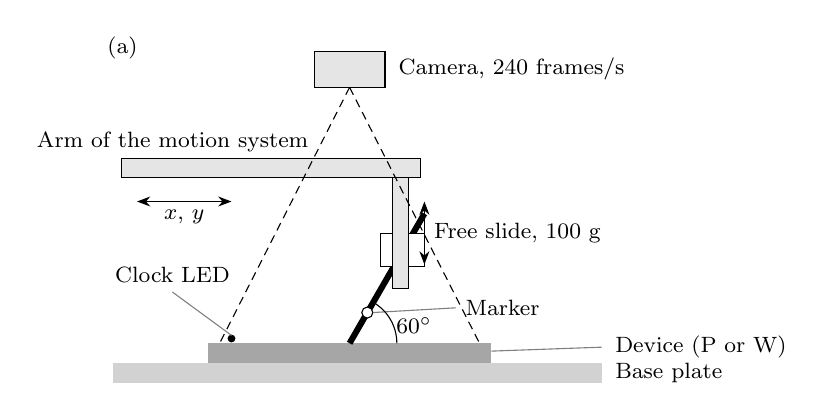
\begin{tikzpicture}[font=\footnotesize, >=Stealth]
% (a) The bench, side view.
\begin{scope}
  \node[anchor=west] at (-0.2,4.25) {(a)};
  \fill[gray!35] (0,0) rectangle (6.2,0.25);
  \node[anchor=west] at (6.25,0.12) {Base plate};
  \fill[gray!70] (1.2,0.25) rectangle (4.8,0.5);
  \node[anchor=west] at (6.25,0.45) {Device (P or W)};
  \draw[gray] (4.8,0.4) -- (6.2,0.45);
  % Stylus at 60 degrees, nib at (3,0.5).
  \draw[line width=2.2pt] (3,0.5) -- ++(60:1.9);
  \fill[white, draw=black] ($(3,0.5)+(60:0.45)$) circle (0.07);
  \draw[gray] ($(3,0.5)+(60:0.45)+(0.07,0)$) -- (4.35,0.95) node[anchor=west, black] {Marker};
  \draw (3.6,0.5) arc (0:60:0.6);
  \node at (3.82,0.72) {$60^\circ$};
  % Holder on a vertical slide.
  \draw[fill=white] ($(3,0.5)+(60:1.35)+(-0.28,-0.2)$) rectangle ++(0.56,0.42);
  \draw[fill=gray!20] (3.55,1.2) rectangle (3.75,2.6);
  \draw[<->] (3.95,1.5) -- (3.95,2.3);
  \node[anchor=west] at (3.95,1.9) {Free slide, 100 g};
  % Plotter arm.
  \draw[fill=gray!20] (0.1,2.6) rectangle (3.9,2.85);
  \node[anchor=east] at (2.6,3.05) {Arm of the motion system};
  \draw[<->] (0.3,2.3) -- (1.5,2.3);
  \node at (0.9,2.1) {$x$, $y$};
  % Camera.
  \draw[fill=gray!20] (2.55,3.75) rectangle (3.45,4.2);
  \node[anchor=west] at (3.5,3.98) {Camera, 240 frames/s};
  \draw[densely dashed] (3,3.75) -- (1.35,0.5);
  \draw[densely dashed] (3,3.75) -- (4.65,0.5);
  % LED.
  \fill (1.5,0.56) circle (0.05);
  \draw[gray] (1.5,0.6) -- (0.75,1.15) node[anchor=south, black] {Clock LED};
\end{scope}
\end{tikzpicture}

\medskip
\begin{tikzpicture}
\begin{groupplot}[group style={group size=3 by 1, horizontal sep=1.25cm},
  height=4.3cm, tick label style={font=\scriptsize}, label style={font=\footnotesize},
  title style={font=\footnotesize}]
\nextgroupplot[width=6.2cm, title={(b) Loops, scale 1.0}, xlabel={$x$ (mm)}, ylabel={$y$ (mm)}, y dir=reverse,
  axis equal image, xmin=0, xmax=112, ymin=0, ymax=28]
\addplot[black, thin] table[x=x, y=y] {figures/path_loops.dat};
\nextgroupplot[width=4.3cm, title={(c) Spiral, scale 1.0}, xlabel={$x$ (mm)}, y dir=reverse,
  axis equal image, xmin=0, xmax=104, ymin=0, ymax=104]
\addplot[black, thin] table[x=x, y=y] {figures/path_spiral.dat};
\nextgroupplot[width=6.2cm, title={(d) Commanded speed}, xlabel={Time (s)}, ylabel={Speed (mm/s)},
  xmin=0, xmax=4, ymin=0, ymax=36, legend style={font=\tiny, at={(0.98,0.03)}, anchor=south east, draw=none, fill=none},
  legend columns=3]
\addplot[black, thin] table[x=t, y=v] {figures/speed_line.dat};
\addplot[black, very thick] table[x=t, y=v] {figures/speed_loops.dat};
\addplot[black, densely dashed, thick] table[x=t, y=v] {figures/speed_spiral.dat};
\legend{Line, Loops, Spiral}
\end{groupplot}
\end{tikzpicture}
\caption{The bench and the movement programs. (a) Side view of the bench. The motion system moves the stylus over the device, which stays still. A free vertical slide sets the load, and the holder sets the angle. The camera above the device tracks a marker near the nib. A clock light (LED) in the field of view gives the frame times. (b), (c) Commanded paths of the loops and the spiral at scale 1.0. (d) Commanded speed during the first four seconds of the loops and the spiral at 20~mm/s and of the line with the 8~Hz oscillation. The figure shows the design, not a measurement.}
\label{fig:bench}
\end{figure}

% This Methods draft needs author verification against both protocols and the executed study.
\section{Methods}
% Budget: 2.5 pages for bench design, devices, programs, features, statistics,
% correction, and the synthetic experiment together.
% Order follows the subsections below. Define each term at its first use.
% This draft states planned procedures. Do not change to past tense without records.
% Leave out implementation paths, tool names, protocol history, and outcome claims.
\pending{Verify all planned procedures against the study records. Confirm the tested hardware, versions, camera settings, and locked program sets.}

\subsection{Devices and fixture}
% Define P, W, run, mounting, and block. Report tested units and software versions.
% Add measured fixture, friction, stiffness, angle, and load values after verification.
Device P is an iPad Pro, M4 or M5, with Apple Pencil Pro.
Device W is a Wacom Intuos Pro Medium (2025), model PTK670, with Pro Pen 3.
The tablet connects to a Mac through USB.
Its active area is $263\times148$ mm, with 200 lines per millimetre \cite{W1}.
The study measures its report rate.
SCRIPT Capture is the iPad recording application; its bench mode records P.
SCRIPT Bench is the Mac recording application; it records W.
\pending{Add both application versions and their release reference.}
A run is one execution of a movement program.
A trial is the recording unit that contains one run.
A mounting is one placement of a device in the fixture.
A block contains all runs of one mounting.

Both devices use bare surfaces and standard new nibs.
Nib replacement occurs at the first and fourth mountings.
A rigid base plate carries the device, motion system, and camera mount.
Edge clamps keep the device flat.
Surface level must be within $0.5^\circ$; axis alignment must be within $1^\circ$.
The holder fixes stylus altitude at $60^\circ$, with the barrel pointing along negative device x.
A free vertical slide applies a total vertical load of 100 g.
Loads must agree within 1 g between devices.
Friction and lateral stiffness measurements must bound nib deflection below 0.02 mm.
A 3 mm white marker on a black field attaches near the nib.
Pressure remains descriptive because the study does not calibrate force.

\subsection{Motion system and programs}
% Define commanded movement and executed movement. Keep the machine choice conditional.
% Add the selected machine and measured settings. Do not state that qualification passed.
The motion system commands prespecified timed movements.
The camera measures the executed movement.
Required travel is at least $152\times124$ mm.
Position resolution must be 0.025 mm or finer, with repeatability of 0.1 mm or better.
Speed accuracy must be within 1\% on a 100 mm line.
The required speed range is 5 to 110 mm/s with the fast loops program.
Required acceleration is at least 3500 mm/s$^2$, or 2000 mm/s$^2$ without that program.
Input shaping is off. Lookahead is off or has a known model.
\pending{Confirm the selected motion system and its measured settings. The candidates are NextDraw 8511 \cite{M3,M4} and Ender-3 V3 KE \cite{M2}.}
A moving device requires a second camera marker fixed to the device.
Camera validation and motion-system acceptance tests must pass before the pilot.

The full main set contains 12 programs.
Loops and spirals use scales of 1.0 and 0.7 at 20 and 40 mm/s.
The full set also includes loops at scale 1.0 and 80 mm/s.
\pending{Confirm whether the motion-system acceptance tests retain the 80 mm/s loops program. Update the program count and run totals.}
Three line programs contain designed oscillations at 5, 8, and 11 Hz.
Their displacement amplitudes are 0.4, 0.25, and 0.18 mm, respectively.
The line cruise speed is 20 mm/s.
Loops follow a curvature-dependent speed profile.
Spiral and line cruise speeds are constant, apart from the designed line oscillations.
Programs use 0.2 s start and end ramps and timed moves sampled every 10 ms.
Each run includes a 0.5 s contact dwell before movement and a 0.3 s dwell after movement.
Each fault program changes loops at scale 1.0 and 20 mm/s after the fourth loop.
The dwell fault adds a 0.5 s stop on the surface.
The lift fault raises the stylus 2 mm at 10 mm/s, waits 0.3 s, then lowers it at 10 mm/s.
The truncation fault ends movement after the fourth loop.

\subsection{Replication and exclusions}
% Define estimability and keep pilot, interim, and main results separate.
Each device has six mountings, with five repeats per main program per mounting.
Each block also contains three repeats of each fault program.
With all 12 main programs, the totals are 720 main runs and 108 fault runs.
The block order is W P P W P W W P W P P W.
Runs follow a fixed random order within each block.
Remounting removes the device and shifts it by at least 10 mm along one axis.
Each mounting repeats axis checks, plane calibration, marker offset measurement, and device qualification tasks.
Device qualification tasks are a 100 mm reference bar, a 10 s still hold, and a 100 mm line at 20 mm/s.

The pilot uses two mountings per device.
It compares each device with its own command, without inspecting between-device feature differences.
Before the main runs, a lock fixes the procedures, limits, program sets, analysis, and recording versions.
The pilot sets the Pencil dwell expectation before this lock.
This expectation specifies whether the dwell gives a contact-gap finding with two contact segments, or no contact-gap finding.
The choice depends on whether the loaded, still Pencil reports samples.
For W, the dwell must give no contact-gap finding.
For this fault, motion duration must be within 2\% of the clean median plus 0.5 s on both devices.
For each measure, the clean median uses valid runs of loops at scale 1.0 and 20 mm/s in the same block.
A lift is detected when the recording contains two contact strokes.
Truncation requires path length and motion duration at most 0.6 times their clean medians.
A fault is detected only when every device-specific criterion holds.

The noise floor is speed power from 4 to 12 Hz when the command contains no such oscillation.
The pilot also fixes eligible band-power programs: the line programs retained for band-power comparison.
On each device, every main line program must produce band power between 0.5 and 2 times its commanded value.
Otherwise, the line programs leave the study before the lock.
Each line program's commanded band power must also reach ten times the larger device noise floor.
A program that fails this rule leaves the band-power comparison set.
After six blocks, an interim check reports variance components only.
If any pooled mounting standard deviation exceeds $0.25L$, two mountings per device are added.
Here $L$ is the feature's equivalence limit.

Nobody compares device feature values until all blocks are complete.
Analysis changes after the lock are reported as post hoc.
\pending{Add the bench lock reference without printing a revision hash. Add the dated consequence registration or equivalent immutable record.}
% Bench protocol section 14 requires the lock commit as the reference.
% Preserve its exact identifier in release metadata, outside the rendered manuscript.

A motion failure means that executed movement fails a camera-to-command check, defined below.
A main run fails after quality rejection, motion failure, or a recorded disturbance or device problem.
Each program has at most two reruns per mounting, used only to replace failures.
A program is estimable for a feature on a device when every mounting has at least four valid runs.
Otherwise, its device difference cannot support an equivalence decision.
Missing camera records exclude runs from camera-referenced comparisons and accuracy analysis.
They do not exclude runs from features without a camera reference.
Every failure, rerun, exclusion, and deviation must be reported.

\subsection{Camera reference and motion interval}
% Define camera-referenced difference. Add actual calibration and validation results later.
The reference requires 240 captured frames per second without frame interpolation.
Pixel scale must be at most 0.12 mm per pixel; exposure must be at most 1 ms.
Length calibration uses a certified grid or a rule with a calibration certificate.
Lens calibration uses at least 20 checkerboard views.
Each mounting uses a marker-plane homography with residual root mean square error at most 0.03 mm.
The marker offset accounts for stylus tilt.
A crystal-timed LED establishes the frame clock.
Rolling-shutter timing requires measured row readout and direction corrections.
Every clip undergoes LED period, frame-time, duplicate-frame, and marker-loss checks.
More than 2\% missing markers invalidates a camera record.
Tracking uses threshold segmentation and an intensity-weighted centroid.

The quality policy splits contact segments at gaps above 0.05 s and requires segments of at least 0.1 s.
It rejects contact sampling below 40 Hz and unresolved estimates.
All tracks use a 200 Hz grid with Savitzky--Golay derivatives, window length 11, and polynomial degree 3.
A qualifying sequence contains six consecutive grid samples with speed at least 2 mm/s.
The motion interval starts at the first sample of the first qualifying sequence.
It ends at the last sample of the last qualifying sequence.
It includes gaps and excludes the contact dwells.
Camera interval detection first uses a command-based alignment window.
Fine alignment maximizes speed-profile correlation and refines the lag below one frame.
Rigid fits use translation and rotation, without scale adjustment.
A maximum camera-to-command path distance above 0.2 mm indicates motion failure.
A motion-duration error above 1\% also indicates motion failure.
So does a camera motion interval that touches its alignment-window edge.
A coarse correlation below 0.5 indicates motion failure when no camera cause explains it.
Camera causes are a short clip or a failed frame-time, frame-integrity, LED-count, or marker-tracking check.

\subsection{Measures, features, and limits}
% Define coefficient of variation, comparison scale, noise floor, and equivalence limit.
% Add full loop segmentation and quality settings if space permits; preserve definitions.
Sampling measures include interval median, interval percentiles, gap share, and hold jitter.
Noise floors use 4 to 12 Hz speed power during still holds and spiral runs.
Spatial accuracy uses camera distances and trace distances from the commanded path.

Speed coefficient of variation (speed CV) is the sample standard deviation of grid speed divided by its mean.
The six primary features are motion duration, smoothed path length, mean speed, loop height, speed CV, and band power.
Path length integrates grid speed over accepted motion segments.
Mean speed averages grid speed within the motion interval.
Loop height is the median height of interior loops.
Baseline points use local vertical maxima with prominence and spacing constraints.
Band power uses Welch spectra in the 4 to 12 Hz band.
Windows last 2 s with half overlap; at least three windows are required.
Duration, path length, and mean speed use all main programs.
Loop height and speed CV use loops only. Band power uses eligible line programs only.

All features use natural logarithms for comparison, except speed CV, which uses its absolute scale.
For four features, each run contributes the device value minus its camera value on the comparison scale.
These features are duration, path length, mean speed, and loop height.
Speed CV and band power use raw device values.
Log dimensionless jerk follows the reported terminology \cite{R3} and remains descriptive.

The limits are $\pm0.036$, $\pm0.044$, $\pm0.044$, $\pm0.047$, $\pm0.030$, and $\pm0.26$, in feature order.
Rule B sets $L=\sqrt{2}\Phi^{-1}(0.55)\sigma_{\mathrm{pop}}$.
Here $\sigma_{\mathrm{pop}}$ is the feature's between-subject standard deviation on its comparison scale.
The function $\Phi$ is the standard normal cumulative distribution function.
Area under the receiver operating characteristic curve is abbreviated AUC.
Under full device confounding with case status, a device bias of $L$ alone gives AUC at most 0.55.
The threshold of 0.55 is a judgment.
Duration and mean-speed limits use published writing measurements \cite{R6}.
Loop height uses writing thickness as a proxy \cite{R4}.
Path length and speed CV use judgment-based limits.
Band power uses a judgment based on tremor-amplitude repeatability in a patient group \cite{R2}.
These sources supply limits; they are not bench participants.
All limits are inclusive and fixed before the main runs.

\subsection{Statistics and correction}
% Define TOST and lack of fit. Do not call the correction check independent validation.
The device bias is P minus W, calculated from program-specific mounting means.
Welch 90\% intervals include mounting variation.
Two one-sided tests (TOST) compare the bias with both limits.
A feature requires equivalence on every program of its prespecified set.
Holm adjustment controls the family across six features at $\alpha=0.05$.
A non-estimable program makes its feature not shown equivalent.
Per-program decisions remain descriptive.
Repeated-measures Bland--Altman summaries report limits for mounting means and single runs.

Correction maps raw W values to raw P values on the comparison scale.
Duration, path length, and mean speed use a Deming model with speed and scale covariates.
Loop height and speed CV use a Deming slope model.
Band power uses a shift model with fixed unit slope.
The covariates are $u=\ln(q/20)$ and $v=\ln(a)$.
Here $q$ is program speed in millimetres per second, and $a$ is geometric scale.
The variance ratio uses mounting and run variance components.
Each mounting pair is omitted in turn to check residual bias against the same limits.
This is a lack-of-fit check with a mounting-based interval, not an independent out-of-sample test.
The full fit supplies the published coefficients; omitted-mounting fits supply jackknife standard errors.
Sensitivities retain motion failures, use raw camera-feature values, group tasks, scales, and speeds, and replace mounting means with medians.
Fault detection and main-run acceptance use exact 95\% Clopper--Pearson intervals.

\subsection{Synthetic consequence experiment}
% Define synthetic participant, observation version, scenario, AUC, calibration, and net benefit.
% Preserve the local-shift assumption. Do not generate W by inverting its fitted correction.
The primary experiments use one feature at a time.
Each cohort contains 600 generated participants, two sessions per participant, and three equally sized sites.
Labels follow a Bernoulli distribution with probability 0.30.
Null and signal effects use standardized mean differences of 0 and 0.8.
Participant and session variation contribute 0.80 and 0.20 of ideal within-class variance.
Each feature's ideal standard deviation is $L/(\sqrt{2}\Phi^{-1}(0.55))$.
This is a simulation assumption, not robot-standardized variation.
Primary cells use 200 independent cohorts; sensitivity cells use 100.

Program selection precedes labels and performance inspection.
It first matches geometry, then minimizes log-distance in scale and speed.
Line selection first minimizes oscillation-frequency distance.
Targets are loops at scale 1.0 and 20 mm/s, and a line at 20 mm/s with 8 Hz oscillation.
Noiseless selected-program features supply the centers.
Unavailable selected inputs remain unavailable.

On the comparison scale, the observation models are
\begin{align}
Z_{P,ij}&=X_{ij}+M_{P,h(i)}+E_{P,ij},\\
Z_{W,ij}&=X_{ij}-b+M_{W,h(i)}+E_{W,ij}.
\end{align}
Here $X$ is the ideal feature, $b$ is the delivered P-minus-W bias, and $M$ and $E$ are Gaussian errors.
Their variances are the delivered mounting and run variances.
Here $i$ identifies a generated participant, and $j$ identifies a session.
The index $h(i)$ identifies the participant's simulation mounting group.
Six device-specific simulation mounting groups remain fixed across sessions.
Transferring camera-referenced bias to raw features assumes that executed-movement differences have been removed.

Reference, uncorrected, and corrected versions share participants, labels, splits, and random draws.
The reference uses P observations throughout.
The uncorrected version uses assigned-device observations.
The corrected version applies the full bench correction to W observations before preprocessing.
Every finite correction is reported diagnostically, including a failed lack-of-fit check.
A correction is bench-supported only when every eligible program residual passes its limit in the omitted-mounting check.
Otherwise, corrected results report failed lack of fit or an unavailable correction.

Scenarios use one device throughout, W-to-P transfer, or device assignment associated with case status.
Transfer assigns each device with probability 0.5, independently of status.
Confounding assigns W with probability 0.85 for cases and 0.15 for controls.
Each participant keeps one device across sessions.
The primary model is L2-regularized logistic regression with inverse regularization strength $C=10$.
It minimizes
\begin{equation}
\overline{\ell}(w)+\frac{\lVert w\rVert^2}{2C},
\end{equation}
where $\overline{\ell}(w)$ is mean log loss and $w$ is the coefficient vector.
Five outer folds and three participant-grouped inner folds support internal validation and Platt calibration.
Imputation and standardization use training data only.
No device, site, mounting, or participant identifier is a predictor.
Separate device-only and site-only baselines assess the information in those assignments.

Record-wise validation permits the same participant in training and testing through different sessions.
It reports this participant overlap.
Participant-wise validation uses participant medians and disjoint participants.
Device-held-out validation also separates devices and reports both transfer directions.
One-device holdout is not applicable; one-class test devices give unavailable metrics.

Metrics include AUC, calibration intercept and slope, Brier score, and decision curves.
AUC compares only within-fold case-control pairs.
Record-wise metrics give each participant total weight one.
Decision curves use thresholds from 0.05 to 0.30 in steps of 0.01, with fold-specific prior-prevalence adjustment.
The target prevalence is 0.30, or 0.08 in the prevalence sensitivity analysis.
Net benefit is a simulation utility, not a clinical recommendation.
For each metric, $D_{\mathrm{raw}}$ is the uncorrected value minus the paired reference value.
The corrected change is the corrected value minus the paired reference value.
Absolute reduction is the absolute raw change minus the absolute corrected change.
A negative absolute reduction indicates worsening.
Signed removal is the raw change minus the corrected change.
Each scenario reports $D_{\mathrm{raw}}$ and absolute reduction for its primary summary.
For one device throughout, this summary is participant-wise AUC for all-W observations against the all-P reference.
For transfer, it is the calibration intercept when training uses W and testing uses P.
For confounding, it is participant-wise AUC under the null effect.

Summaries separate simulation distribution intervals from Monte Carlo uncertainty in mean contrasts.
They report metric-specific denominators, failures, material-change shares, and incomplete cells.
A material change has an absolute reference difference of at least 0.05 for AUC or 0.20 log-odds for calibration intercept.
The thresholds are 0.20 for estimable calibration slopes and 0.01 for mean net benefit across the decision thresholds.
These are descriptive judgments.
Cells with fewer than 95\% of their planned paired replicates are marked incomplete.
This requires at least 190 usable pairs in primary cells and 95 in sensitivity cells.
Measured analyses condition on delivered point estimates.
Bias-bound sensitivities do not propagate joint bench-estimation uncertainty.
The assumed grid uses $b=kL$, with $k\in\{-2,-1,-0.5,0,0.5,1,2\}$.
Noise settings specify session-error and mounting-error standard deviations, each divided by $L$.
Zero noise assigns $(0,0)$ to both devices.
Nominal noise assigns P $(0.25,0.10)$ and W $(0.25,0.25)$.
Stress noise assigns P $(0.25,0.25)$ and W $(0.50,0.50)$.
The oracle correction adds the known shift $b$ and leaves random noise unchanged.
A grid-only misspecified-correction control uses nominal noise at $k=-1,0,1$.
Let $c$ be the selected program's noiseless center on the comparison scale.
Slope-capable controls set slope $1.05$ and intercept $b+0.5L-0.05c$.
Shift controls keep slope 1 and set intercept $b+0.5L$.
All grid correction covariates have zero coefficients.
Both misspecified controls therefore have error $0.5L$ at $c$, relative to the oracle correction.
These assumed controls are reported separately from measured inputs.
Sensitivity analyses change one setting at a time.
Grid sensitivities use $k=-1,0,1$ with nominal noise; measured sensitivities keep the delivered bias and noise.
They use cohort sizes of 200 or 1200, prevalence 0.08, signal effect 0.4, or participant variance share 0.95.
Further checks use all six independent features, nearest-neighbor prediction, or independent and fully confounded device assignments.
Nearest-neighbor checks select among 15, 5, and 1 neighbors by inner-fold AUC.
Negative generated speed CV values remain in primary analyses, with their frequency reported.
A separate sensitivity floors observed speed CV at zero before correction.
No result establishes human reliability, screening accuracy, or clinical utility.

\section{Results}
% Budget: 2.3 pages, including all main tables and figures.
% Order: data completeness; sampling and accuracy; feature agreement;
% correction; quality gate; synthetic consequences and validation diagnostics.
% Define estimable, adjusted decision, correction support, and unavailable estimate.
% Do not insert numbers until outputs exist. Include every planned result.
% Claim rules: bench protocol section 16 and consequence protocol section 11.
% A feature claim needs all prespecified programs and the Holm-adjusted decision.
% Camera references apply only to duration, path length, mean speed, and loop height.
% Speed CV and band power concern commanded movement within the executed-motion check.
% Keep per-program results descriptive. A failed test does not prove a difference.
% Correction residuals are a lack-of-fit check, not independent transfer validation.
% Separate grid assumptions from measured-input consequences throughout.
% Do not claim human agreement, reliability, screening accuracy, or clinical utility.

\subsection{Completeness, sampling, and accuracy}
\pending{R-completeness: report valid runs, failures, reruns, missing camera records, deviations, and non-estimable programs.}
\begin{table}[t]
% Caption specification: State the observed sampling and accuracy pattern within the tested range.
% Show device and program summaries for sample intervals, gap shares, noise floors, camera distances, and command trace error.
% Give units, valid-run counts, and ranges.
\caption{}
\label{tab:sampling}
\pending{T-sampling: insert the sampling and spatial accuracy table. Write the caption from its specification.}
\end{table}
\pending{R-sampling: describe measured sampling and accuracy without an acceptance claim. Include hold sample counts and camera validity.}

\subsection{Feature agreement}
\begin{table}[t]
% Caption specification: State which features meet the prespecified equivalence decision across their full program sets.
% Show limits, comparison scales, camera-reference status, feature p-values, adjusted and unadjusted decisions, and estimability.
% Keep per-program decisions descriptive.
\caption{}
\label{tab:agreement}
\pending{T-agreement: insert all feature decisions, including failures. Write the caption from its specification.}
\end{table}
\begin{figure}[t]
\pending{F-agreement: insert the bias intervals and repeated-measures agreement plots. Write the caption from its specification.}
% Caption specification: State the observed pattern of bias relative to the prespecified limits.
% Show program-specific intervals and Bland--Altman points with mounting-mean and single-run limits of agreement.
% Identify comparison scales and the camera-referenced features.
\caption{}
\label{fig:agreement}
\end{figure}
\pending{R-agreement: state only supported feature-level decisions. Report per-program bias and sensitivity results as descriptive evidence.}

\subsection{Correction and quality gate}
\begin{table}[t]
% Caption specification: State whether each correction passes its lack-of-fit check across every prespecified program.
% Show model terms, fitted or fixed status, coefficient uncertainty, and omitted-mounting residual intervals against the same limits.
% Do not describe these intervals as independent validation.
\caption{}
\label{tab:correction}
\pending{T-correction: insert coefficients, residuals, and support status. Write the caption from its specification.}
\end{table}
\pending{R-correction: report residual sizes, failed checks, and unavailable fits. Bound use to the tested measurement chain and range.}
\begin{table}[t]
% Caption specification: State which designed faults the quality gate detects on each device.
% Show main-run acceptance and detection by fault and device, with exact intervals and denominators.
% State the locked Pencil dwell expectation.
\caption{}
\label{tab:gate}
\pending{T-gate: insert acceptance and fault-detection summaries. Write the caption from its specification.}
\end{table}
\pending{R-gate: describe each fault outcome. Do not infer detection of untested faults.}

\subsection{Synthetic consequences}
\begin{table}[t]
% Caption specification: State the scenario-specific primary changes from the paired synthetic reference.
% Show raw change, corrected change, absolute reduction, uncertainty, material-change share, usable pairs, and correction support for every feature.
% Primary summaries: participant-wise AUC for all-W against all-P; W-to-P calibration
% intercept for transfer; participant-wise AUC under the null effect for confounding.
% Report D_raw and absolute reduction, as defined in Methods, for each summary.
% Separate assumed grids from measured inputs.
\caption{}
\label{tab:consequence}
\pending{T-consequence: insert the primary consequence summaries and write the caption from its specification.}
\end{table}
\begin{figure}[t]
\pending{F-consequence: insert bias-response, transfer-calibration, and decision-curve panels. Write the caption from its specification.}
% Caption specification: State how the measurement-chain difference changes synthetic model metrics under the specified assumptions.
% Show uncorrected and corrected bias response, directional transfer calibration, and decision curves against paired references.
% Distinguish mean uncertainty from simulation distribution intervals. Retain unavailable levels and corrections that worsen results.
\caption{}
\label{fig:consequence}
\end{figure}
% Report the target geometry, scale, speed, frequency, and selected program for every feature.
% Put scale-and-speed distance beside absolute frequency difference. State range status.
% Mark extrapolation as sensitivity evidence. Do not select programs by performance.
\pending{R-program-selection: report the selected programs, target settings, both distances, and range status.}
\pending{R-consequence: report the scenario-specific primary metrics and all supporting metrics. Explain negative absolute reductions and incomplete cells.}
\pending{R-validation: compare record-wise, participant-wise, and both device-held-out directions. Report overlap, baselines, refusals, and sensitivity analyses.}
% State beside the affected results that path length, speed CV, and band-power population
% scaling has no independent population justification. Joint features are not one drawing.
% A small synthetic effect does not establish equivalence. No numerical lower bound
% on human AUC or calibration distortion follows from omitted surface behavior.
% Optional example: omit by default. Add a separate result only after written clearance,
% public provenance, participant grouping, deduplication, and full citations are verified.

\section{Discussion}
% Budget: discussion, limitations, and statements share 0.9 page.
% Order: answer each measurement question from supported results; explain correction
% failure or success; explain chain-only synthetic consequences; state limitations;
% close with the evidence needed before any use with people.
% Define lack of fit and conditional simulation uncertainty in reader-facing terms.
% Leave out project history, health associations, deployment advice, and human claims.
\pending{Interpret each feature decision and correction result within the tested range. Explain synthetic consequences under their stated assumptions.}

\subsection{Limitations}
% Write one limitations paragraph. Cover one tested unit of each device; software,
% surfaces, mountings, angle, azimuth, load, active region, sizes, and speeds.
% Explain that a robot cannot measure changes in human movement caused by surfaces.
% Cite R6 for the surface effect. The correction addresses only measurement-chain error.
% Band power concerns designed line oscillations only. Jerk, pressure, tilt, and hover
% are descriptive. The camera is not a band-power or instantaneous-timing reference.
% Explain conservative feature decisions and limited power without treating failure
% as proof of a difference. Explain that omitted-mounting checks assess lack of fit.
% Synthetic Gaussian feature assumptions, local-shift transfer, population scaling,
% independent joint features, and fixed bench estimates constrain interpretation.
% Simulation intervals exclude bench-estimation uncertainty. Behavioral and chain
% effects can oppose each other. Do not state a numerical lower bound for people.
\pending{Write the limitations paragraph. Explain the surface effect \cite{R6} and each bound on inference.}

\section*{Data and code availability}
\pending{Before submission: place the recordings, the camera tracks, the programs, the lock record, the analysis code, and the capture applications in a repository with an anonymous review link, and give the link here. State the licences. Until the release exists, this statement makes no promise.}

\section*{Ethics}
The study has no participants.
It uses no data from people.
The consequence experiment uses generated cohorts only.
The equivalence limits use summary values from published studies.

\section*{Use of artificial intelligence tools}
\pending{The authors must complete this disclosure, check it against the policy of the journal, and name the tools and versions.}
Under the direction of the authors, generative artificial intelligence tools (large language models) wrote drafts of the capture and analysis software, of its tests, of the study protocols, and of this manuscript, and reviewed them.
The authors reviewed and verified all code, analyses, and text, checked every reference against its source, and take full responsibility for the content.
% Acknowledgements, funding, and competing interests are withheld for double-anonymous review.
% Add them after acceptance.

\bibliographystyle{unsrtnat}
\bibliography{references}
\end{document}
